\chapter{最短路径}

\index{最短路径}

在图中寻找两个节点之间的最短路径
是一个重要的问题，有着许多
实际应用。
例如，与道路网络相关的一个自然问题是，
在给定各条道路长度的情况下，
计算两座城市之间路线的最短可能长度。

在无权图中，路径的长度等于
其边的数量，我们可以
简单地使用广度优先搜索来找到
最短路径。
然而，在本章中我们关注的是
带权图，
其中需要更复杂的算法
来寻找最短路径。

\section{Bellman–Ford算法}

\index{Bellman–Ford算法}

\key{Bellman–Ford算法}\footnote{该算法以
R. E. Bellman 和 L. R. Ford 的名字命名，
他们分别于
1958年和1956年独立发表了该算法 \cite{bel58,for56a}。}用于寻找
从起始节点到图中所有节点的
最短路径。
该算法可以处理各种类型的图，
前提是图中不包含
长度为负的环。
如果图中包含负环，
该算法也能检测出来。

该算法跟踪从起始节点到图中所有节点的距离。
初始时，到起始节点的距离为0，
到所有其他节点的距离为无穷大。
算法通过找到
能够缩短路径的边来减小距离，
直到无法再减小任何距离为止。

\subsubsection{示例}

让我们考虑Bellman–Ford算法
在以下图中的工作过程：
\begin{center}
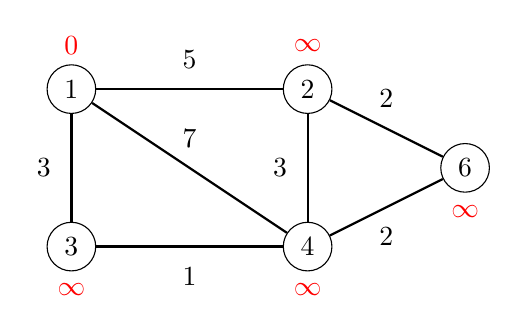
\begin{tikzpicture}
\node[draw, circle] (1) at (1,3) {1};
\node[draw, circle] (2) at (4,3) {2};
\node[draw, circle] (3) at (1,1) {3};
\node[draw, circle] (4) at (4,1) {4};
\node[draw, circle] (5) at (6,2) {6};
\node[color=red] at (1,3+0.55) {$0$};
\node[color=red] at (4,3+0.55) {$\infty$};
\node[color=red] at (1,1-0.55) {$\infty$};
\node[color=red] at (4,1-0.55) {$\infty$};
\node[color=red] at (6,2-0.55) {$\infty$};
\path[draw,thick,-] (1) -- node[font=\small,label=above:5] {} (2);
\path[draw,thick,-] (1) -- node[font=\small,label=left:3] {} (3);
\path[draw,thick,-] (3) -- node[font=\small,label=below:1] {} (4);
\path[draw,thick,-] (2) -- node[font=\small,label=left:3] {} (4);
\path[draw,thick,-] (2) -- node[font=\small,label=above:2] {} (5);
\path[draw,thick,-] (4) -- node[font=\small,label=below:2] {} (5);
\path[draw,thick,-] (1) -- node[font=\small,label=above:7] {} (4);
\end{tikzpicture}
\end{center}
图中的每个节点都被赋予一个距离。
初始时，到起始节点的距离为0，
到所有其他节点的距离为无穷大。

算法搜索能够减小距离的边。
首先，从节点1出发的所有边减小了距离：
\begin{center}
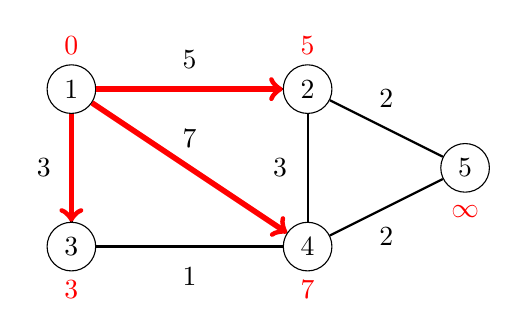
\begin{tikzpicture}
\node[draw, circle] (1) at (1,3) {1};
\node[draw, circle] (2) at (4,3) {2};
\node[draw, circle] (3) at (1,1) {3};
\node[draw, circle] (4) at (4,1) {4};
\node[draw, circle] (5) at (6,2) {5};
\node[color=red] at (1,3+0.55) {$0$};
\node[color=red] at (4,3+0.55) {$5$};
\node[color=red] at (1,1-0.55) {$3$};
\node[color=red] at (4,1-0.55) {$7$};
\node[color=red] at (6,2-0.55) {$\infty$};
\path[draw,thick,-] (1) -- node[font=\small,label=above:5] {} (2);
\path[draw,thick,-] (1) -- node[font=\small,label=left:3] {} (3);
\path[draw,thick,-] (3) -- node[font=\small,label=below:1] {} (4);
\path[draw,thick,-] (2) -- node[font=\small,label=left:3] {} (4);
\path[draw,thick,-] (2) -- node[font=\small,label=above:2] {} (5);
\path[draw,thick,-] (4) -- node[font=\small,label=below:2] {} (5);
\path[draw,thick,-] (1) -- node[font=\small,label=above:7] {} (4);

\path[draw=red,thick,->,line width=2pt] (1) -- (2);
\path[draw=red,thick,->,line width=2pt] (1) -- (3);
\path[draw=red,thick,->,line width=2pt] (1) -- (4);
\end{tikzpicture}
\end{center}
之后，边
$2 \rightarrow 5$ 和 $3 \rightarrow 4$
减小了距离：
\begin{center}
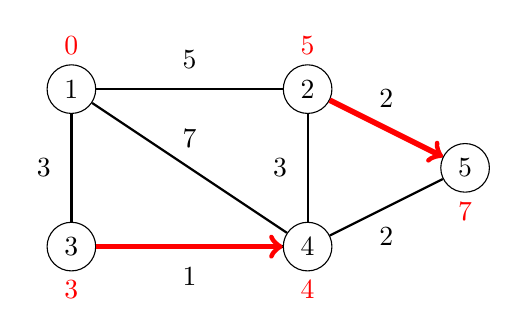
\begin{tikzpicture}
\node[draw, circle] (1) at (1,3) {1};
\node[draw, circle] (2) at (4,3) {2};
\node[draw, circle] (3) at (1,1) {3};
\node[draw, circle] (4) at (4,1) {4};
\node[draw, circle] (5) at (6,2) {5};
\node[color=red] at (1,3+0.55) {$0$};
\node[color=red] at (4,3+0.55) {$5$};
\node[color=red] at (1,1-0.55) {$3$};
\node[color=red] at (4,1-0.55) {$4$};
\node[color=red] at (6,2-0.55) {$7$};
\path[draw,thick,-] (1) -- node[font=\small,label=above:5] {} (2);
\path[draw,thick,-] (1) -- node[font=\small,label=left:3] {} (3);
\path[draw,thick,-] (3) -- node[font=\small,label=below:1] {} (4);
\path[draw,thick,-] (2) -- node[font=\small,label=left:3] {} (4);
\path[draw,thick,-] (2) -- node[font=\small,label=above:2] {} (5);
\path[draw,thick,-] (4) -- node[font=\small,label=below:2] {} (5);
\path[draw,thick,-] (1) -- node[font=\small,label=above:7] {} (4);

\path[draw=red,thick,->,line width=2pt] (2) -- (5);
\path[draw=red,thick,->,line width=2pt] (3) -- (4);
\end{tikzpicture}
\end{center}
最后，还有一次变化：
\begin{center}
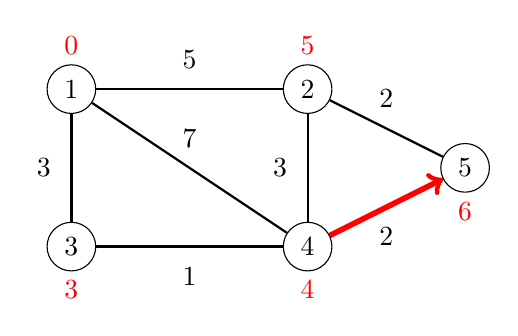
\begin{tikzpicture}
\node[draw, circle] (1) at (1,3) {1};
\node[draw, circle] (2) at (4,3) {2};
\node[draw, circle] (3) at (1,1) {3};
\node[draw, circle] (4) at (4,1) {4};
\node[draw, circle] (5) at (6,2) {5};
\node[color=red] at (1,3+0.55) {$0$};
\node[color=red] at (4,3+0.55) {$5$};
\node[color=red] at (1,1-0.55) {$3$};
\node[color=red] at (4,1-0.55) {$4$};
\node[color=red] at (6,2-0.55) {$6$};
\path[draw,thick,-] (1) -- node[font=\small,label=above:5] {} (2);
\path[draw,thick,-] (1) -- node[font=\small,label=left:3] {} (3);
\path[draw,thick,-] (3) -- node[font=\small,label=below:1] {} (4);
\path[draw,thick,-] (2) -- node[font=\small,label=left:3] {} (4);
\path[draw,thick,-] (2) -- node[font=\small,label=above:2] {} (5);
\path[draw,thick,-] (4) -- node[font=\small,label=below:2] {} (5);
\path[draw,thick,-] (1) -- node[font=\small,label=above:7] {} (4);

\path[draw=red,thick,->,line width=2pt] (4) -- (5);
\end{tikzpicture}
\end{center}

此后，没有任何边能减小任何距离。
这意味着距离已经是最终的，
我们已经成功计算出了
从起始节点到图中所有节点的
最短距离。

例如，从节点1到节点5的最短距离3
对应以下路径：

\begin{center}
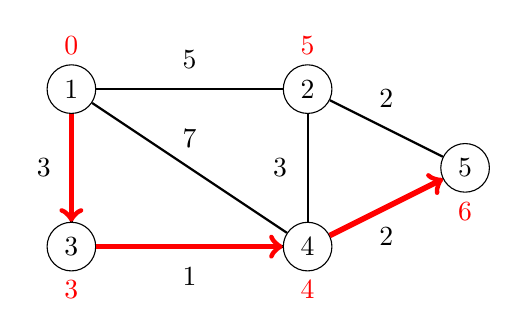
\begin{tikzpicture}
\node[draw, circle] (1) at (1,3) {1};
\node[draw, circle] (2) at (4,3) {2};
\node[draw, circle] (3) at (1,1) {3};
\node[draw, circle] (4) at (4,1) {4};
\node[draw, circle] (5) at (6,2) {5};
\node[color=red] at (1,3+0.55) {$0$};
\node[color=red] at (4,3+0.55) {$5$};
\node[color=red] at (1,1-0.55) {$3$};
\node[color=red] at (4,1-0.55) {$4$};
\node[color=red] at (6,2-0.55) {$6$};
\path[draw,thick,-] (1) -- node[font=\small,label=above:5] {} (2);
\path[draw,thick,-] (1) -- node[font=\small,label=left:3] {} (3);
\path[draw,thick,-] (3) -- node[font=\small,label=below:1] {} (4);
\path[draw,thick,-] (2) -- node[font=\small,label=left:3] {} (4);
\path[draw,thick,-] (2) -- node[font=\small,label=above:2] {} (5);
\path[draw,thick,-] (4) -- node[font=\small,label=below:2] {} (5);
\path[draw,thick,-] (1) -- node[font=\small,label=above:7] {} (4);

\path[draw=red,thick,->,line width=2pt] (1) -- (3);
\path[draw=red,thick,->,line width=2pt] (3) -- (4);
\path[draw=red,thick,->,line width=2pt] (4) -- (5);
\end{tikzpicture}
\end{center}

\subsubsection{实现}

以下是Bellman–Ford算法的实现，
用于确定从节点$x$到图中所有节点的最短距离。
代码假设图以边列表 \texttt{edges} 的形式存储，
其中每个元素是形如 $(a,b,w)$ 的元组，
表示从节点 $a$ 到节点 $b$ 有一条
权重为 $w$ 的边。

算法由 $n-1$ 轮组成，
每轮算法遍历
图中的所有边并尝试
减小距离。
算法构建一个数组 \texttt{distance}，
其中包含从 $x$ 
到图中所有节点的距离。
常量 \texttt{INF} 表示无穷大的距离。

\begin{lstlisting}
for (int i = 1; i <= n; i++) distance[i] = INF;
distance[x] = 0;
for (int i = 1; i <= n-1; i++) {
    for (auto e : edges) {
        int a, b, w;
        tie(a, b, w) = e;
        distance[b] = min(distance[b], distance[a]+w);
    }
}
\end{lstlisting}

算法的时间复杂度为 $O(nm)$，
因为算法由 $n-1$ 轮组成，
每轮迭代所有 $m$ 条边。
如果图中没有负环，
所有距离在 $n-1$ 轮后即为最终值，
因为每条最短路径最多包含 $n-1$ 条边。

在实际应用中，最终距离通常
可以比 $n-1$ 轮更快地找到。
因此，提高算法效率的一种可能方法
是在某轮中没有任何距离能被减小
时停止算法。

\subsubsection{负环}

\index{负环}

Bellman–Ford算法也可以用来
检查图中是否包含长度为负的环。
例如，图

\begin{center}
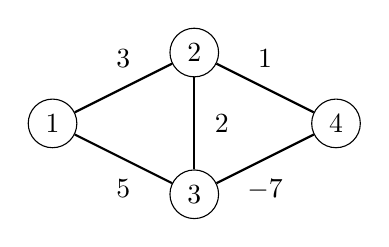
\begin{tikzpicture}[scale=0.9]
\node[draw, circle] (1) at (0,0) {$1$};
\node[draw, circle] (2) at (2,1) {$2$};
\node[draw, circle] (3) at (2,-1) {$3$};
\node[draw, circle] (4) at (4,0) {$4$};

\path[draw,thick,-] (1) -- node[font=\small,label=above:$3$] {} (2);
\path[draw,thick,-] (2) -- node[font=\small,label=above:$1$] {} (4);
\path[draw,thick,-] (1) -- node[font=\small,label=below:$5$] {} (3);
\path[draw,thick,-] (3) -- node[font=\small,label=below:$-7$] {} (4);
\path[draw,thick,-] (2) -- node[font=\small,label=right:$2$] {} (3);
\end{tikzpicture}
\end{center}
\noindent
包含一个负环
$2 \rightarrow 3 \rightarrow 4 \rightarrow 2$，
其长度为 $-4$。

如果图中包含负环，
对于任何包含该环的路径，
我们可以通过不断重复该环
来无限次地缩短路径。
因此，在这种情况下，
最短路径的概念
是没有意义的。

可以通过运行Bellman–Ford算法 $n$ 轮
来检测负环。
如果最后一轮减小了任何距离，
则图中包含负环。
注意，该算法可用于
在整个图中搜索
负环，
与起始节点的选择无关。

\subsubsection{SPFA算法}

\index{SPFA算法}

\key{SPFA算法}（''Shortest Path Faster Algorithm''，最短路径更快算法）\cite{fan94}
是Bellman–Ford算法的一个变体，
通常比原始算法更高效。
SPFA算法不会每轮遍历所有边，
而是以更智能的方式
选择要检查的边。

算法维护一个可能
用于减小距离的节点队列。
首先，算法将起始节点 $x$
加入队列。
然后，算法总是处理
队列中的第一个节点，当边
$a \rightarrow b$ 减小了某个距离时，
节点 $b$ 被加入队列。
% 
% 以下实现使用了一个
% \texttt{queue} \texttt{q}。
% 此外，数组 \texttt{inqueue} 指示
% 一个节点是否已在队列中，
% 如果在，则算法不会再次
% 将该节点加入队列。
% 
% \begin{lstlisting}
% for (int i = 1; i <= n; i++) distance[i] = INF;
% distance[x] = 0;
% q.push(x);
% while (!q.empty()) {
%     int a = q.front(); q.pop();
%     inqueue[a] = false;
%     for (auto b : v[a]) {
%         if (distance[a]+b.second < distance[b.first]) {
%             distance[b.first] = distance[a]+b.second;
%             if (!inqueue[b]) {q.push(b); inqueue[b] = true;}
%         }
%     }
% }
% \end{lstlisting}

SPFA算法的效率取决于
图的结构：
该算法通常很高效，
但其最坏情况时间复杂度仍为
$O(nm)$，并且可以构造出
使算法与原始Bellman–Ford算法一样慢的输入。

\section{Dijkstra算法}

\index{Dijkstra算法}

\key{Dijkstra算法}\footnote{E. W. Dijkstra 于1959年发表了该算法 \cite{dij59}；
然而，他的原始论文并未提及如何高效地实现该算法。}
与Bellman–Ford算法一样，
用于寻找
从起始节点到图中所有节点的最短路径。
Dijkstra算法的优点是
它更高效，可以用于
处理大型图。
但是，该算法要求图中
不存在负权边。

与Bellman–Ford算法类似，
Dijkstra算法维护到各节点的距离，
并在搜索过程中减小它们。
Dijkstra算法之所以高效，是因为
它利用不存在负边这一事实，
只处理图中的每条边一次。

\subsubsection{示例}

让我们考虑当
起始节点为节点1时，Dijkstra算法
在以下图中的工作过程：
\begin{center}
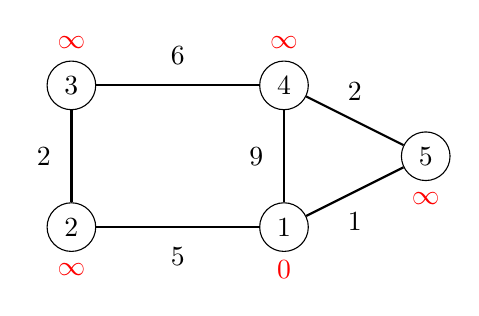
\begin{tikzpicture}[scale=0.9]
\node[draw, circle] (1) at (1,3) {3};
\node[draw, circle] (2) at (4,3) {4};
\node[draw, circle] (3) at (1,1) {2};
\node[draw, circle] (4) at (4,1) {1};
\node[draw, circle] (5) at (6,2) {5};

\node[color=red] at (1,3+0.6) {$\infty$};
\node[color=red] at (4,3+0.6) {$\infty$};
\node[color=red] at (1,1-0.6) {$\infty$};
\node[color=red] at (4,1-0.6) {$0$};
\node[color=red] at (6,2-0.6) {$\infty$};

\path[draw,thick,-] (1) -- node[font=\small,label=above:6] {} (2);
\path[draw,thick,-] (1) -- node[font=\small,label=left:2] {} (3);
\path[draw,thick,-] (3) -- node[font=\small,label=below:5] {} (4);
\path[draw,thick,-] (2) -- node[font=\small,label=left:9] {} (4);
\path[draw,thick,-] (2) -- node[font=\small,label=above:2] {} (5);
\path[draw,thick,-] (4) -- node[font=\small,label=below:1] {} (5);
\end{tikzpicture}
\end{center}
与Bellman–Ford算法一样，
初始时到起始节点的距离为0，
到所有其他节点的距离为无穷大。

在每一步中，Dijkstra算法选择一个
尚未被处理且距离
尽可能小的节点。
第一个这样的节点是距离为0的节点1。

当一个节点被选中后，算法
遍历从该节点出发的所有边，
并利用它们来减小距离：
\begin{center}
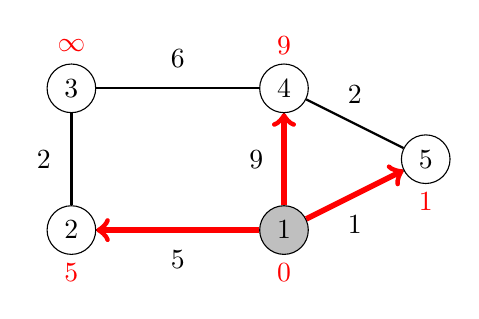
\begin{tikzpicture}[scale=0.9]
\node[draw, circle] (1) at (1,3) {3};
\node[draw, circle] (2) at (4,3) {4};
\node[draw, circle] (3) at (1,1) {2};
\node[draw, circle, fill=lightgray] (4) at (4,1) {1};
\node[draw, circle] (5) at (6,2) {5};

\node[color=red] at (1,3+0.6) {$\infty$};
\node[color=red] at (4,3+0.6) {$9$};
\node[color=red] at (1,1-0.6) {$5$};
\node[color=red] at (4,1-0.6) {$0$};
\node[color=red] at (6,2-0.6) {$1$};

\path[draw,thick,-] (1) -- node[font=\small,label=above:6] {} (2);
\path[draw,thick,-] (1) -- node[font=\small,label=left:2] {} (3);
\path[draw,thick,-] (3) -- node[font=\small,label=below:5] {} (4);
\path[draw,thick,-] (2) -- node[font=\small,label=left:9] {} (4);
\path[draw,thick,-] (2) -- node[font=\small,label=above:2] {} (5);
\path[draw,thick,-] (4) -- node[font=\small,label=below:1] {} (5);

\path[draw=red,thick,->,line width=2pt] (4) -- (2);
\path[draw=red,thick,->,line width=2pt] (4) -- (3);
\path[draw=red,thick,->,line width=2pt] (4) -- (5);
\end{tikzpicture}
\end{center}
在这种情况下，
从节点1出发的边减小了
节点2、4和5的距离，它们的距离现在是5、9和1。

下一个要处理的节点是距离为1的节点5。
这将节点4的距离从9减小到3：
\begin{center}
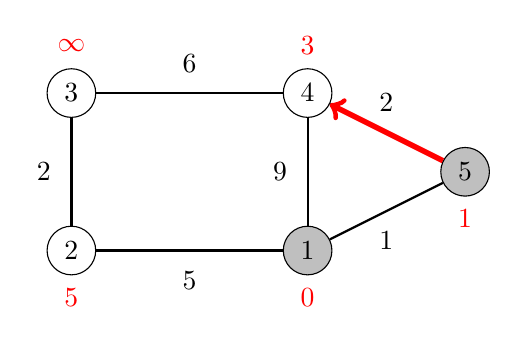
\begin{tikzpicture}
\node[draw, circle] (1) at (1,3) {3};
\node[draw, circle] (2) at (4,3) {4};
\node[draw, circle] (3) at (1,1) {2};
\node[draw, circle, fill=lightgray] (4) at (4,1) {1};
\node[draw, circle, fill=lightgray] (5) at (6,2) {5};

\node[color=red] at (1,3+0.6) {$\infty$};
\node[color=red] at (4,3+0.6) {$3$};
\node[color=red] at (1,1-0.6) {$5$};
\node[color=red] at (4,1-0.6) {$0$};
\node[color=red] at (6,2-0.6) {$1$};

\path[draw,thick,-] (1) -- node[font=\small,label=above:6] {} (2);
\path[draw,thick,-] (1) -- node[font=\small,label=left:2] {} (3);
\path[draw,thick,-] (3) -- node[font=\small,label=below:5] {} (4);
\path[draw,thick,-] (2) -- node[font=\small,label=left:9] {} (4);
\path[draw,thick,-] (2) -- node[font=\small,label=above:2] {} (5);
\path[draw,thick,-] (4) -- node[font=\small,label=below:1] {} (5);

\path[draw=red,thick,->,line width=2pt] (5) -- (2);
\end{tikzpicture}
\end{center}
之后，下一个节点是节点4，
它将节点3的距离减小到9：
\begin{center}
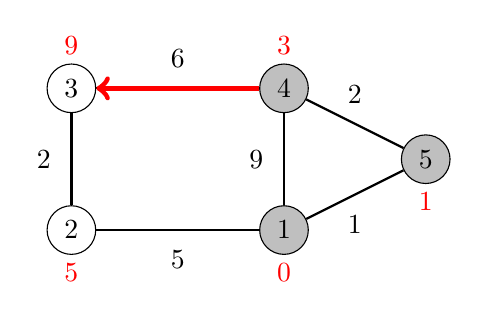
\begin{tikzpicture}[scale=0.9]
\node[draw, circle] (1) at (1,3) {3};
\node[draw, circle, fill=lightgray] (2) at (4,3) {4};
\node[draw, circle] (3) at (1,1) {2};
\node[draw, circle, fill=lightgray] (4) at (4,1) {1};
\node[draw, circle, fill=lightgray] (5) at (6,2) {5};

\node[color=red] at (1,3+0.6) {$9$};
\node[color=red] at (4,3+0.6) {$3$};
\node[color=red] at (1,1-0.6) {$5$};
\node[color=red] at (4,1-0.6) {$0$};
\node[color=red] at (6,2-0.6) {$1$};

\path[draw,thick,-] (1) -- node[font=\small,label=above:6] {} (2);
\path[draw,thick,-] (1) -- node[font=\small,label=left:2] {} (3);
\path[draw,thick,-] (3) -- node[font=\small,label=below:5] {} (4);
\path[draw,thick,-] (2) -- node[font=\small,label=left:9] {} (4);
\path[draw,thick,-] (2) -- node[font=\small,label=above:2] {} (5);
\path[draw,thick,-] (4) -- node[font=\small,label=below:1] {} (5);

\path[draw=red,thick,->,line width=2pt] (2) -- (1);
\end{tikzpicture}
\end{center}

Dijkstra算法的一个显著特性是，
每当一个节点被选中时，其距离就是最终的。
例如，在算法的这个时刻，
距离0、1和3分别是到
节点1、5和4的最终距离。

此后，算法处理剩余的两个
节点，最终距离如下：

\begin{center}
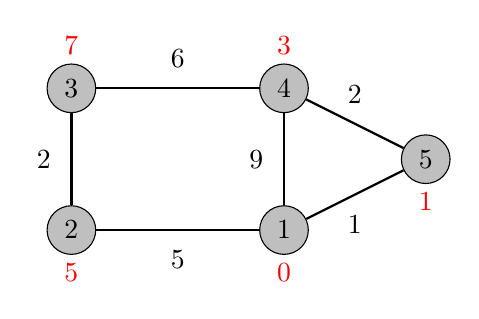
\begin{tikzpicture}[scale=0.9]
\node[draw, circle, fill=lightgray] (1) at (1,3) {3};
\node[draw, circle, fill=lightgray] (2) at (4,3) {4};
\node[draw, circle, fill=lightgray] (3) at (1,1) {2};
\node[draw, circle, fill=lightgray] (4) at (4,1) {1};
\node[draw, circle, fill=lightgray] (5) at (6,2) {5};

\node[color=red] at (1,3+0.6) {$7$};
\node[color=red] at (4,3+0.6) {$3$};
\node[color=red] at (1,1-0.6) {$5$};
\node[color=red] at (4,1-0.6) {$0$};
\node[color=red] at (6,2-0.6) {$1$};

\path[draw,thick,-] (1) -- node[font=\small,label=above:6] {} (2);
\path[draw,thick,-] (1) -- node[font=\small,label=left:2] {} (3);
\path[draw,thick,-] (3) -- node[font=\small,label=below:5] {} (4);
\path[draw,thick,-] (2) -- node[font=\small,label=left:9] {} (4);
\path[draw,thick,-] (2) -- node[font=\small,label=above:2] {} (5);
\path[draw,thick,-] (4) -- node[font=\small,label=below:1] {} (5);
\end{tikzpicture}
\end{center}

\subsubsection{负边}

Dijkstra算法的效率
基于图中不包含
负边这一事实。
如果存在负边，
算法可能给出错误的结果。
举例来说，考虑以下图：

\begin{center}
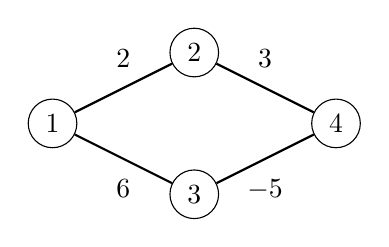
\begin{tikzpicture}[scale=0.9]
\node[draw, circle] (1) at (0,0) {$1$};
\node[draw, circle] (2) at (2,1) {$2$};
\node[draw, circle] (3) at (2,-1) {$3$};
\node[draw, circle] (4) at (4,0) {$4$};

\path[draw,thick,-] (1) -- node[font=\small,label=above:2] {} (2);
\path[draw,thick,-] (2) -- node[font=\small,label=above:3] {} (4);
\path[draw,thick,-] (1) -- node[font=\small,label=below:6] {} (3);
\path[draw,thick,-] (3) -- node[font=\small,label=below:$-5$] {} (4);
\end{tikzpicture}
\end{center}
\noindent
从节点1到节点4的最短路径是
$1 \rightarrow 3 \rightarrow 4$，
其长度为1。
然而，Dijkstra算法
通过跟随最小权重的边
找到了路径 $1 \rightarrow 2 \rightarrow 4$。
算法没有考虑到，
在另一条路径上，权重 $-5$
可以补偿之前的大权重 $6$。

\subsubsection{实现}

以下是Dijkstra算法的实现，
计算从节点 $x$ 到图中其他节点的最小距离。
图以邻接表的形式存储，
即当从节点 $a$ 到节点 $b$ 有一条
权重为 $w$ 的边时，\texttt{adj[$a$]} 包含一个对 $(b,w)$。

Dijkstra算法的高效实现
要求能够高效地找到
尚未处理的最小距离节点。
适合的数据结构是优先队列，
其中包含按距离排序的节点。
使用优先队列，下一个要处理的节点
可以在对数时间内取出。

在以下代码中，优先队列
\texttt{q} 包含形如 $(-d,x)$ 的对，
表示到节点 $x$ 的当前距离为 $d$。
数组 $\texttt{distance}$ 包含到
每个节点的距离，数组 $\texttt{processed}$ 指示
一个节点是否已被处理。
初始时，到 $x$ 的距离为 $0$，到所有其他节点的距离为 $\infty$。

\begin{lstlisting}
for (int i = 1; i <= n; i++) distance[i] = INF;
distance[x] = 0;
q.push({0,x});
while (!q.empty()) {
    int a = q.top().second; q.pop();
    if (processed[a]) continue;
    processed[a] = true;
    for (auto u : adj[a]) {
        int b = u.first, w = u.second;
        if (distance[a]+w < distance[b]) {
            distance[b] = distance[a]+w;
            q.push({-distance[b],b});
        }
    }
}
\end{lstlisting}

注意，优先队列中包含节点的\emph{负}
距离。
原因是C++默认版本的优先队列查找最大
元素，而我们希望找到最小元素。
通过使用负距离，
我们可以直接使用默认的优先队列\footnote{当然，
我们也可以像第4.5章中那样声明优先队列
并使用正距离，但实现会稍长一些。}。
还需要注意的是，优先队列中可能存在同一节点的多个实例；
然而，只有距离最小的实例会被处理。

上述实现的时间复杂度为
$O(n+m \log m)$，因为算法遍历
图中的所有节点，并且为每条边
最多向优先队列添加一个距离。

\section{Floyd–Warshall算法}

\index{Floyd–Warshall算法}

\key{Floyd–Warshall算法}\footnote{该算法
以 R. W. Floyd 和 S. Warshall 的名字命名，
他们于1962年独立发表了该算法 \cite{flo62,war62}。}
提供了一种解决
最短路径问题的替代方法。
与本章的其他算法不同，
它在一次运行中找到节点之间的
所有最短路径。

算法维护一个二维数组，
其中包含节点之间的距离。
首先，仅使用
节点之间的直接边来计算距离，
之后，算法通过在路径中使用中间节点
来减小距离。

\subsubsection{示例}

让我们考虑Floyd–Warshall算法
在以下图中的工作过程：

\begin{center}
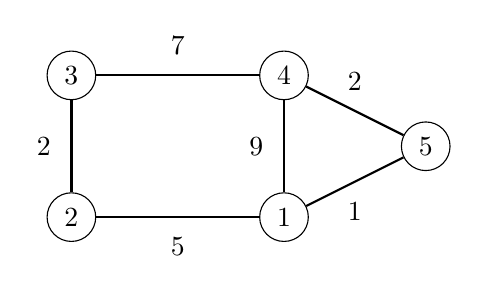
\begin{tikzpicture}[scale=0.9]
\node[draw, circle] (1) at (1,3) {$3$};
\node[draw, circle] (2) at (4,3) {$4$};
\node[draw, circle] (3) at (1,1) {$2$};
\node[draw, circle] (4) at (4,1) {$1$};
\node[draw, circle] (5) at (6,2) {$5$};

\path[draw,thick,-] (1) -- node[font=\small,label=above:7] {} (2);
\path[draw,thick,-] (1) -- node[font=\small,label=left:2] {} (3);
\path[draw,thick,-] (3) -- node[font=\small,label=below:5] {} (4);
\path[draw,thick,-] (2) -- node[font=\small,label=left:9] {} (4);
\path[draw,thick,-] (2) -- node[font=\small,label=above:2] {} (5);
\path[draw,thick,-] (4) -- node[font=\small,label=below:1] {} (5);
\end{tikzpicture}
\end{center}

初始时，每个节点到自身的距离为 $0$，
如果节点 $a$ 和节点 $b$ 之间有一条
权重为 $x$ 的边，则它们之间的距离为 $x$。
所有其他距离为无穷大。

在这个图中，初始数组如下：
\begin{center}
\begin{tabular}{r|rrrrr}
 & 1 & 2 & 3 & 4 & 5 \\
\hline
1 & 0 & 5 & $\infty$ & 9 & 1 \\
2 & 5 & 0 & 2 & $\infty$ & $\infty$ \\
3 & $\infty$ & 2 & 0 & 7 & $\infty$ \\
4 & 9 & $\infty$ & 7 & 0 & 2 \\
5 & 1 & $\infty$ & $\infty$ & 2 & 0 \\
\end{tabular}
\end{center}
\vspace{10pt}
算法由连续的轮次组成。
在每一轮中，算法选择一个新节点
作为路径中的中间节点，
并利用该节点来减小距离。

在第一轮中，节点1是新的中间节点。
节点2和节点4之间出现了一条
长度为14的新路径，因为节点1连接了它们。
节点2和节点5之间也出现了一条
长度为6的新路径。

\begin{center}
\begin{tabular}{r|rrrrr}
 & 1 & 2 & 3 & 4 & 5 \\
\hline
1 & 0 & 5 & $\infty$ & 9 & 1 \\
2 & 5 & 0 & 2 & \textbf{14} & \textbf{6} \\
3 & $\infty$ & 2 & 0 & 7 & $\infty$ \\
4 & 9 & \textbf{14} & 7 & 0 & 2 \\
5 & 1 & \textbf{6} & $\infty$ & 2 & 0 \\
\end{tabular}
\end{center}
\vspace{10pt}

在第二轮中，节点2是新的中间节点。
这创建了节点1和节点3之间
以及节点3和节点5之间的新路径：

\begin{center}
\begin{tabular}{r|rrrrr}
 & 1 & 2 & 3 & 4 & 5 \\
\hline
1 & 0 & 5 & \textbf{7} & 9 & 1 \\
2 & 5 & 0 & 2 & 14 & 6 \\
3 & \textbf{7} & 2 & 0 & 7 & \textbf{8} \\
4 & 9 & 14 & 7 & 0 & 2 \\
5 & 1 & 6 & \textbf{8} & 2 & 0 \\
\end{tabular}
\end{center}
\vspace{10pt}

在第三轮中，节点3是新的中间节点。
节点2和节点4之间出现了一条新路径：

\begin{center}
\begin{tabular}{r|rrrrr}
 & 1 & 2 & 3 & 4 & 5 \\
\hline
1 & 0 & 5 & 7 & 9 & 1 \\
2 & 5 & 0 & 2 & \textbf{9} & 6 \\
3 & 7 & 2 & 0 & 7 & 8 \\
4 & 9 & \textbf{9} & 7 & 0 & 2 \\
5 & 1 & 6 & 8 & 2 & 0 \\
\end{tabular}
\end{center}
\vspace{10pt}

算法继续这样进行，
直到所有节点都被指定为中间节点。
算法结束后，数组包含
任意两个节点之间的最小距离：

\begin{center}
\begin{tabular}{r|rrrrr}
 & 1 & 2 & 3 & 4 & 5 \\
\hline
1 & 0 & 5 & 7 & 3 & 1 \\
2 & 5 & 0 & 2 & 8 & 6 \\
3 & 7 & 2 & 0 & 7 & 8 \\
4 & 3 & 8 & 7 & 0 & 2 \\
5 & 1 & 6 & 8 & 2 & 0 \\
\end{tabular}
\end{center}

例如，数组告诉我们
节点2和节点4之间的最短距离为8。
这对应以下路径：

\begin{center}
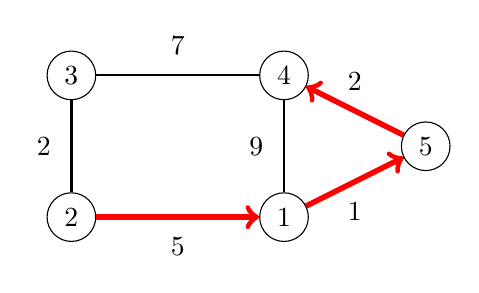
\begin{tikzpicture}[scale=0.9]
\node[draw, circle] (1) at (1,3) {$3$};
\node[draw, circle] (2) at (4,3) {$4$};
\node[draw, circle] (3) at (1,1) {$2$};
\node[draw, circle] (4) at (4,1) {$1$};
\node[draw, circle] (5) at (6,2) {$5$};

\path[draw,thick,-] (1) -- node[font=\small,label=above:7] {} (2);
\path[draw,thick,-] (1) -- node[font=\small,label=left:2] {} (3);
\path[draw,thick,-] (3) -- node[font=\small,label=below:5] {} (4);
\path[draw,thick,-] (2) -- node[font=\small,label=left:9] {} (4);
\path[draw,thick,-] (2) -- node[font=\small,label=above:2] {} (5);
\path[draw,thick,-] (4) -- node[font=\small,label=below:1] {} (5);

\path[draw=red,thick,->,line width=2pt] (3) -- (4);
\path[draw=red,thick,->,line width=2pt] (4) -- (5);
\path[draw=red,thick,->,line width=2pt] (5) -- (2);
\end{tikzpicture}
\end{center}

\subsubsection{实现}

Floyd–Warshall算法的优点是
它易于实现。
以下代码构造一个
距离矩阵，其中 $\texttt{distance}[a][b]$
是节点 $a$ 和 $b$ 之间的最短距离。
首先，算法使用图的邻接矩阵 \texttt{adj}
来初始化 \texttt{distance}：

\begin{lstlisting}
for (int i = 1; i <= n; i++) {
    for (int j = 1; j <= n; j++) {
        if (i == j) distance[i][j] = 0;
        else if (adj[i][j]) distance[i][j] = adj[i][j];
        else distance[i][j] = INF;
    }
}
\end{lstlisting}
此后，最短距离可以如下求得：
\begin{lstlisting}
for (int k = 1; k <= n; k++) {
    for (int i = 1; i <= n; i++) {
        for (int j = 1; j <= n; j++) {
            distance[i][j] = min(distance[i][j],
                                   distance[i][k]+distance[k][j]);
        }
    }
}
\end{lstlisting}

算法的时间复杂度为 $O(n^3)$，
因为它包含三个嵌套循环
来遍历图中的节点。

由于Floyd–Warshall算法的实现简单，
即使只需要在图中找一条
最短路径，该算法也可以是
一个不错的选择。
然而，该算法只能在图足够小、
使得立方时间复杂度足够快时使用。
